\chapter{Background and State of the Art}

This chapter reviews previous tethered satellite missions and the current state of the art in optical reconstruction methods for slender structures. The objective is to establish the technological and methodological context that motivates the development of the LINKU stereo vision system.
\\\\
The chapter first analyzes the observational limitations encountered in previous tethered missions, particularly regarding the lack of direct geometric visualization of the deployed tether. Subsequently, the chapter reviews the theoretical foundations of conventional photogrammetry, the limitations of texture-based reconstruction under orbital conditions, and alternative approaches based on geometric extraction and emerging AI-assisted methods.
\\\\
Through this analysis, the chapter identifies the principal technological gap addressed by the LINKU project, the absence of a dedicated stereo reconstruction approach specifically adapted to thin, textureless tether structures observed under high-contrast orbital illumination.

\section{Lessons from previous tethered missions}

Several tethered satellite missions have demonstrated the scientific and technological relevance of tether systems in orbit, including applications related to electrodynamic propulsion, gravity-gradient stabilization, orbital dynamics characterization, and formation control. However, despite these advances, direct visual reconstruction of deployed tether geometry has remained a major unresolved challenge.
\\\\
Historically, most tethered missions relied primarily on indirect telemetry measurements or limited visual inspection capabilities rather than on dedicated geometric reconstruction systems. Consequently, the actual spatial configuration of the tether during deployment and post-deployment operations could not always be directly characterized, particularly under dynamic or anomalous conditions.
\\\\
In the context of nano- and micro-satellites, the STARS-II mission developed by Kagawa University demonstrated the deployment concept of an electrodynamic tether between a Mother Satellite (MS) and a Daughter Satellite (DS), as illustrated in Figure \ref{fig:figure2.1}. \cite{nohmi2014stars}. This mission validated the feasibility of tether deployment within a nanosatellite architecture and demonstrated the operational relevance of tethered systems for future orbital applications.
\\\\
However, despite the relevance of this architecture, STARS-II did not incorporate a dedicated visual reconstruction capability to directly estimate the three-dimensional geometry of the tether during flight operations. Due to operational limitations and the absence of dedicated optical instrumentation, deployment analysis relied primarily on indirect observations derived from orbital behavior and telemetry interpretation.
\\\\
While these measurements provided valuable mission-level information, they did not allow direct observation of tether curvature, oscillatory behavior, localized deformation, or deployment anomalies throughout the extension process.

\begin{figure}[!ht]
    \centering
    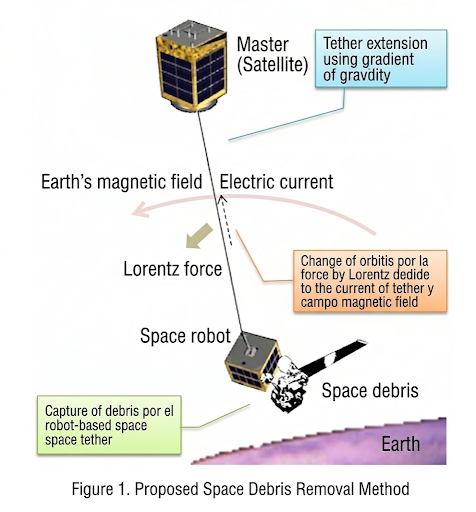
\includegraphics[width=0.5\textwidth]{Images/Figure 2.1.png}
    \caption[Conceptual configuration of the STARS-II mission]{Conceptual configuration of the STARS-II mission, illustrating the Mother Satellite (MS) and Daughter Satellite (DS) connected by an electrodynamic tether (EDT) \cite{nohmi2014stars}.}
    \label{fig:figure2.1}
\end{figure}

Similar observational limitations were present in larger tether missions such as NASA's TSS-1 and TSS-1R programs. Although these missions incorporated onboard imaging systems for operational monitoring, they did not include a dedicated stereo-vision architecture designed for geometric tether reconstruction.
\\\\
When the tether failed during the TSS-1R mission, the available visual data were insufficient to directly characterize the full structural dynamics of the rupture event. As a result, post-flight analysis relied heavily on telemetry interpretation and indirect estimation methods derived from dynamic models and flight data.
\\\\
These precedents highlight a common technological limitation in previous tethered missions: the lack of dedicated visual systems capable of continuously reconstructing the tether's three-dimensional geometry under orbital conditions. This limitation becomes particularly critical when characterizing transient oscillations, local deformations, deployment anomalies, or out-of-plane motion.
\\\\
These observational limitations motivate the need to evaluate reconstruction methods specifically adapted to the optical and geometric conditions expected during orbital tether observation.

\section{Theoretical basis and reconstruction of slender structures}

The optical reconstruction of thin structures presents a fundamentally different problem compared to the conventional three-dimensional reconstruction of volumetric objects. Standard photogrammetry techniques were originally developed for textured surfaces observed under diffuse illumination, where stable visual features can be extracted and matched across multiple images.
\\\\
However, tether reconstruction in orbit introduces a combination of constraints that significantly complicates the use of traditional feature-based methods:

\begin{itemize}
    \item Extremely thin geometry
    \item Limited or nonexistent surface texture
    \item Strong directional illumination.
    \item High radiometric contrast
    \item Predominantly featureless backgrounds
\end{itemize}

Under these conditions, the tether may occupy only a fraction of a pixel at long observation distances, while simultaneously lacking distinguishable surface patterns required for conventional feature matching.
\\\\
For this reason, the reconstruction problem addressed in the LINKU mission must be treated primarily as a geometric and radiometric detection problem rather than as a conventional texture-matching problem.

\subsection{Standard photogrammetry and its limitations}

Traditional photogrammetry is based on the extraction and correspondence of visual features between multiple images. Methods such as Structure-from-Motion (SfM) and Semi-Global Matching (SGM) estimate three-dimensional geometry by matching textured image regions observed from different viewpoints.
\\\\
These methods operate effectively when the observed scene contains:
\begin{itemize}
    \item Stable texture patterns
    \item Diffuse illumination
    \item Sufficient spatial contrast
    \item Volumetric structures occupying multiple pixels
\end{itemize}

Under terrestrial conditions, surrounding environmental texture and ambient illumination help stabilize the feature-matching process. However, the orbital environment expected for tether observation differs substantially from these assumptions.
\\\\
In the LINKU observation scenario, the tether is expected to appear as a thin, nearly textureless structure against a low-radiance background. Under these conditions, conventional feature descriptors cannot reliably identify stable correspondences between stereo images.
\\\\
Additionally, highly directional solar illumination may produce localized specular reflections and saturation effects that violate the brightness-consistency assumptions typically required by standard photogrammetry algorithms \cite{kniaz2020wire, yu2023bonding}.
\\\\
As observation distance increases, the tether projection may also enter the sub-pixel regime, where the apparent width of the structure becomes smaller than a single image pixel. In this regime, traditional patch-based stereo correspondence methods become fundamentally unreliable because the target no longer occupies a sufficiently large image region for stable feature extraction.
\\\\
These limitations become particularly critical under representative high-contrast orbital-like imaging conditions, where conventional photogrammetry struggles to maintain reliable feature correspondence for thin tether structures.
\\\\
Figure \ref{fig:figure2.2} reflects the fundamental limitation identified by Kniaz et al. \cite{kniaz2020wire}, conventional image-based reconstruction methods rely heavily on stable visual features and texture-rich observations. As the observed structure becomes thinner and less textured, feature correspondence becomes increasingly unreliable, motivating the development of alternative reconstruction approaches based on geometric continuity, radiometric analysis, and line-based representations rather than traditional texture-based feature matching.
\newpage
\clearpage

\begin{figure}[!ht]
    \centering
    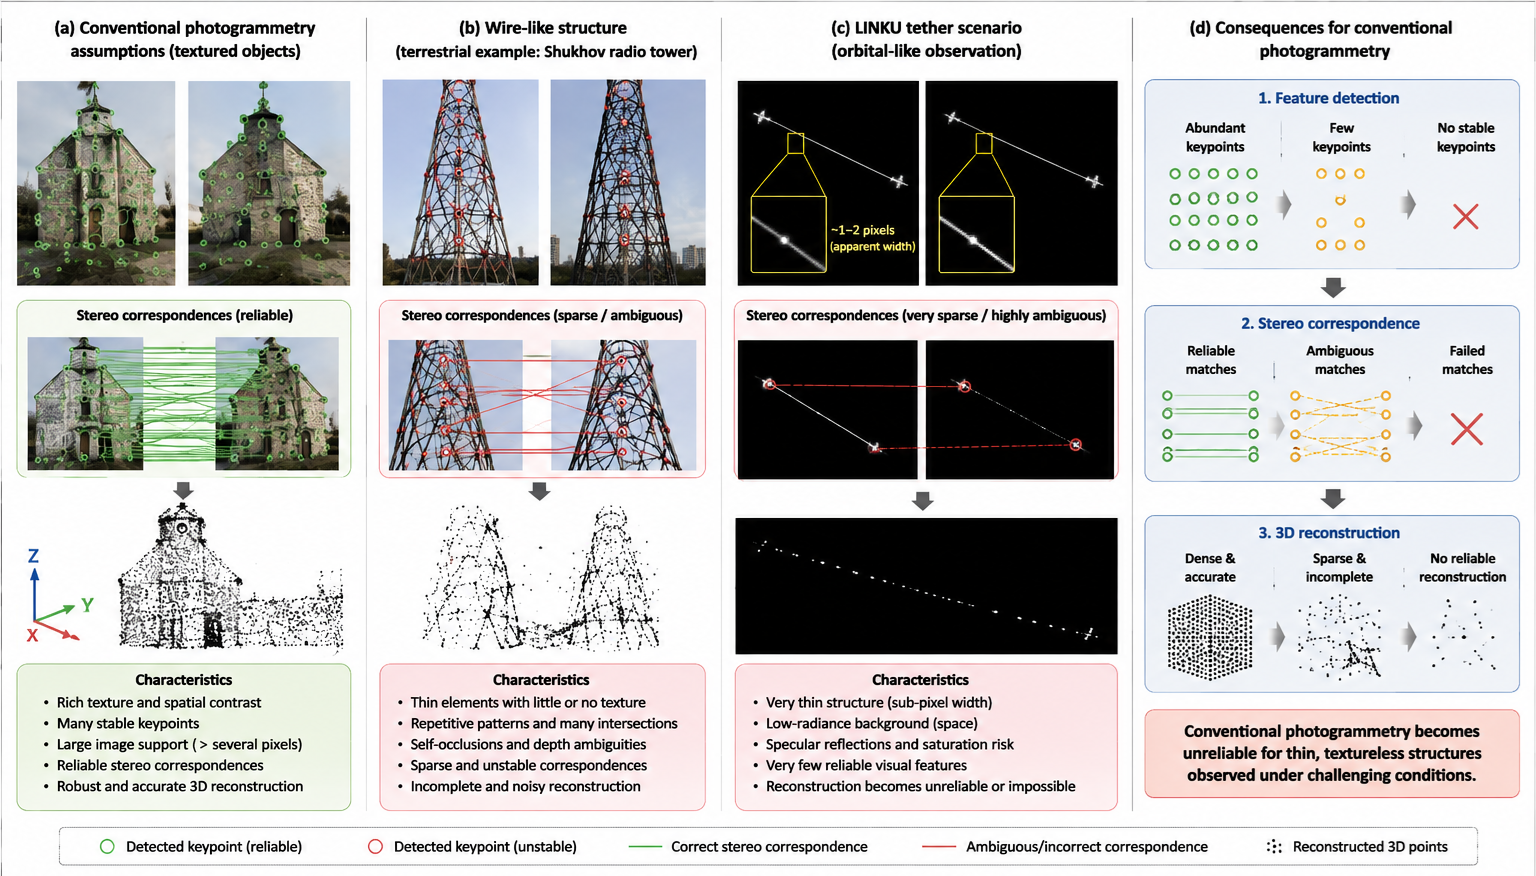
\includegraphics[width=\textwidth]{Images/Figure 2.2.png}
    \caption[Conceptual illustration of the challenges associated with conventional photogrammetry when applied to thin wire-like structures and orbital tether observation]{Conceptual illustration of the challenges associated with conventional photogrammetry when applied to thin wire-like structures and orbital tether observation, inspired by the reconstruction limitations discussed by Kniaz et al. \cite{kniaz2020wire}. (a) presents a conventional photogrammetry scenario, where textured surfaces provide a large number of stable visual features that can be reliably detected and matched between images. Under these conditions, Structure-from-Motion (SfM) and stereo reconstruction algorithms can establish dense correspondences and generate accurate three-dimensional reconstructions. (b) illustrates a wire-like structure, where the available visual information is significantly reduced due to the thin geometry and repetitive patterns. As a result, the number of distinctive features decreases and correspondence ambiguity increases. (c) represents the orbital tether observation scenario considered in LINKU, where the tether appears as a thin, low-texture structure observed against a dark background under directional illumination. In this regime, the tether may occupy only a few pixels or even operate under sub-pixel conditions, further reducing the availability of reliable feature descriptors. (d) summarizes the consequences for conventional photogrammetry, showing the progressive degradation of feature detection, stereo correspondence, and three-dimensional reconstruction performance as the scene transitions from textured objects to thin wire-like and tether-like structures.}
    \label{fig:figure2.2}
\end{figure}

\subsection{Edge-based extraction: Alternative for textureless geometry}

Because texture-based correspondence becomes unreliable for thin structures, alternative reconstruction strategies must rely primarily on geometric contrast rather than on surface texture.
\\\\
In terrestrial industrial inspection applications, edge-based and centerline-based extraction methods are commonly used to detect slender structures such as metallic wires, filaments, or bonding traces \cite{yu2023bonding}. Instead of identifying textured image patches, these methods estimate the geometric location of the structure boundary or centerline relative to the surrounding background.
\\\\
This approach is particularly relevant for the LINKU mission because the tether is expected to appear primarily as a radiometric line-like feature rather than as a textured object.
\\\\
Sub-pixel line extraction methods, such as those derived from Steger's framework \cite{steger2000subpixel}, provide a mathematical basis for estimating the centerline position of thin structures, even when the apparent width approaches the pixel-resolution limit. These methods exploit intensity gradients and scale-space analysis to estimate geometric location with sub-pixel precision.
\\\\
For the LINKU stereo vision system, these principles provide the theoretical foundation for a reconstruction approach centered on:

\begin{itemize}
    \item Tether segmentation
    \item Centerline estimation
    \item Stereo geometric correspondence
    \item Curve-based triangulation
\end{itemize}

By focusing on geometric continuity and radiometric contrast rather than texture matching, the proposed approach is more compatible with the expected optical conditions for orbital tether observation.
\\\\
As shown in Figure \ref{fig:figure2.3}, the presented workflow follows the principles established by Steger \cite{steger2000subpixel}, in which line-like structures are not characterized by texture-based features but by their radiometric profiles, gradient behavior, and sub-pixel localization properties. This interpretation is particularly relevant for orbital tether observation, where the target may occupy only a few pixels or even operate within the sub-pixel regime, making conventional feature-based photogrammetry unreliable.

\begin{figure}[!ht]
    \centering
    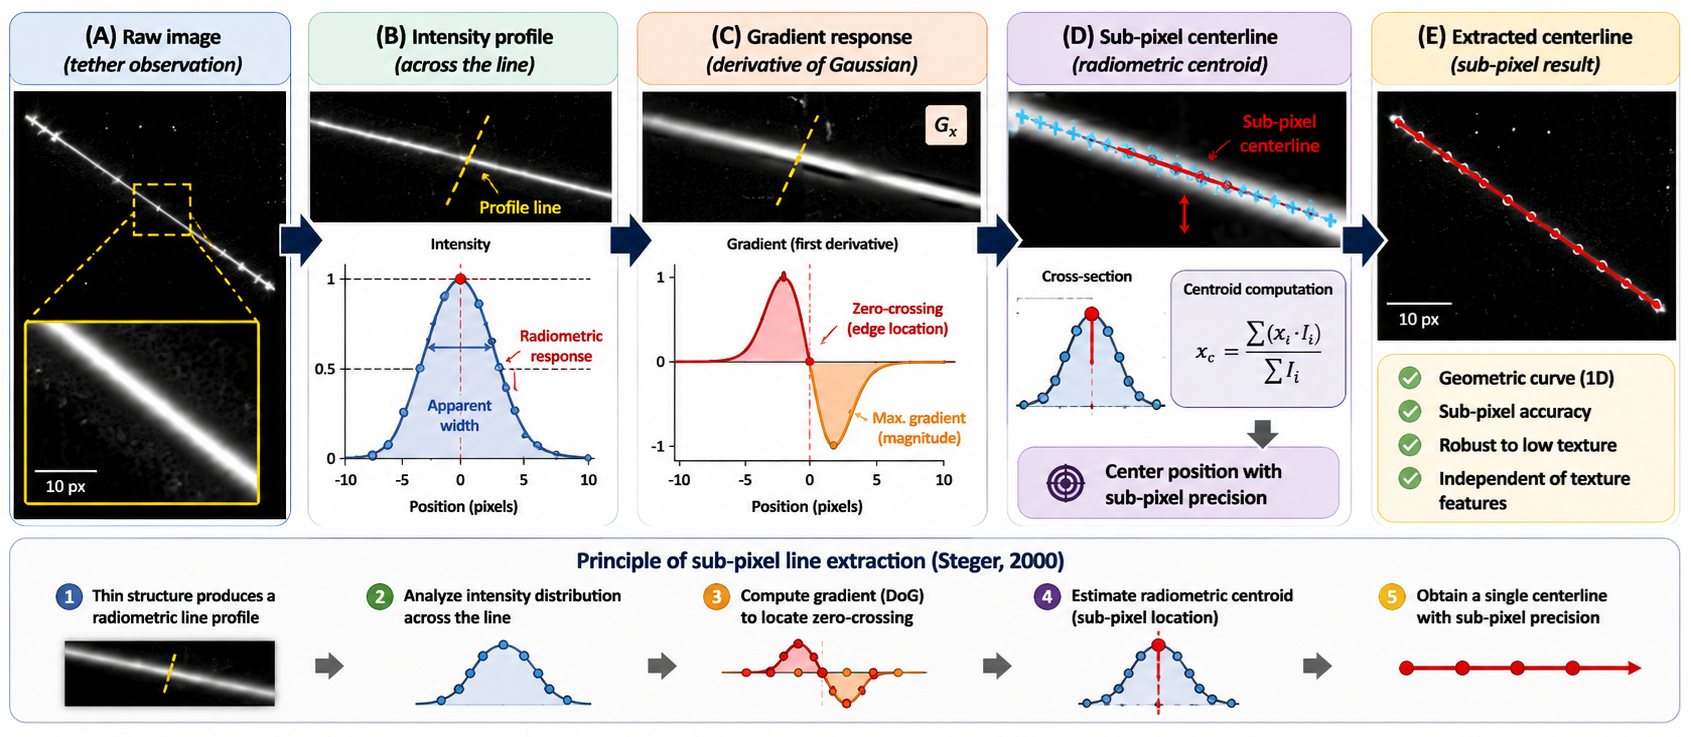
\includegraphics[width=\textwidth]{Images/Figure 2.3.png}
    \caption[Conceptual illustration of the sub-pixel line extraction process for thin structures based on the line-profile interpretation framework proposed by Steger \cite{steger2000subpixel}]{Conceptual illustration of the sub-pixel line extraction process for thin structures based on the line-profile interpretation framework proposed by Steger \cite{steger2000subpixel}. (A) shows the raw image of a thin tether-like structure, which appears as a finite-width radiometric response due to the combined effects of the optical system, sensor sampling, and image blur. (B) illustrates the intensity profile extracted across the line, where the structure is represented by a localized radiometric distribution rather than a perfectly resolved geometric object. (C) presents the corresponding gradient response, obtained via derivative-based filtering, which reveals the intensity transitions associated with the line boundaries and provides information on line localization. (D) shows the estimation of the line center using radiometric centroiding and sub-pixel localization, enabling inference of the centerline position with precision greater than the sensor pixel spacing. Finally, (E) presents the extracted centerline representation, where the thin structure is reduced to a single geometric trajectory suitable for subsequent curve tracking, stereo correspondence, and three-dimensional reconstruction.}
    \label{fig:figure2.3}
\end{figure}

\subsection{The limitations of emerging AI methods for space}

Recent advances in Artificial Intelligence (AI), including convolutional neural networks (CNNs), neural rendering methods, and Neural Radiance Fields (NeRFs), have demonstrated promising capabilities for image segmentation and three-dimensional reconstruction in terrestrial environments \cite{kniaz2020wire,xie2019pix2vox,melas2023realfusion}.
\\\\
These approaches can outperform traditional reconstruction methods when large representative datasets and stable imaging conditions are available. However, their direct application to orbital tether observation remains highly challenging.
\\\\
Most currently available datasets used for AI-based reconstruction contain textured objects, ambient illumination, structured environments, and dense visual context. In contrast, the LINKU observation scenario involves highly directional illumination, extreme background contrast, sparse visual reference, and thin sub-pixel structures.
\\\\
This mismatch between terrestrial training datasets and the expected orbital environment limits the direct applicability of current AI-based approaches.
\\\\
Additionally, many neural reconstruction methods require substantial computational resources that are not compatible with lightweight onboard processing constraints typically associated with nanosatellite platforms.
\\\\
For these reasons, AI-assisted reconstruction is treated within the LINKU project as an exploratory future-oriented capability intended to complement, rather than replace, the primary geometry-driven reconstruction approach.
\\\\
Figure \ref{fig:figure2.4} illustrates the contrast between contemporary AI-assisted reconstruction scenarios and the orbital tether observation conditions considered in LINKU. This comparison highlights the domain gap that currently limits the direct application of AI-based reconstruction methods to the proposed mission.

\begin{figure}[!ht]
    \centering
    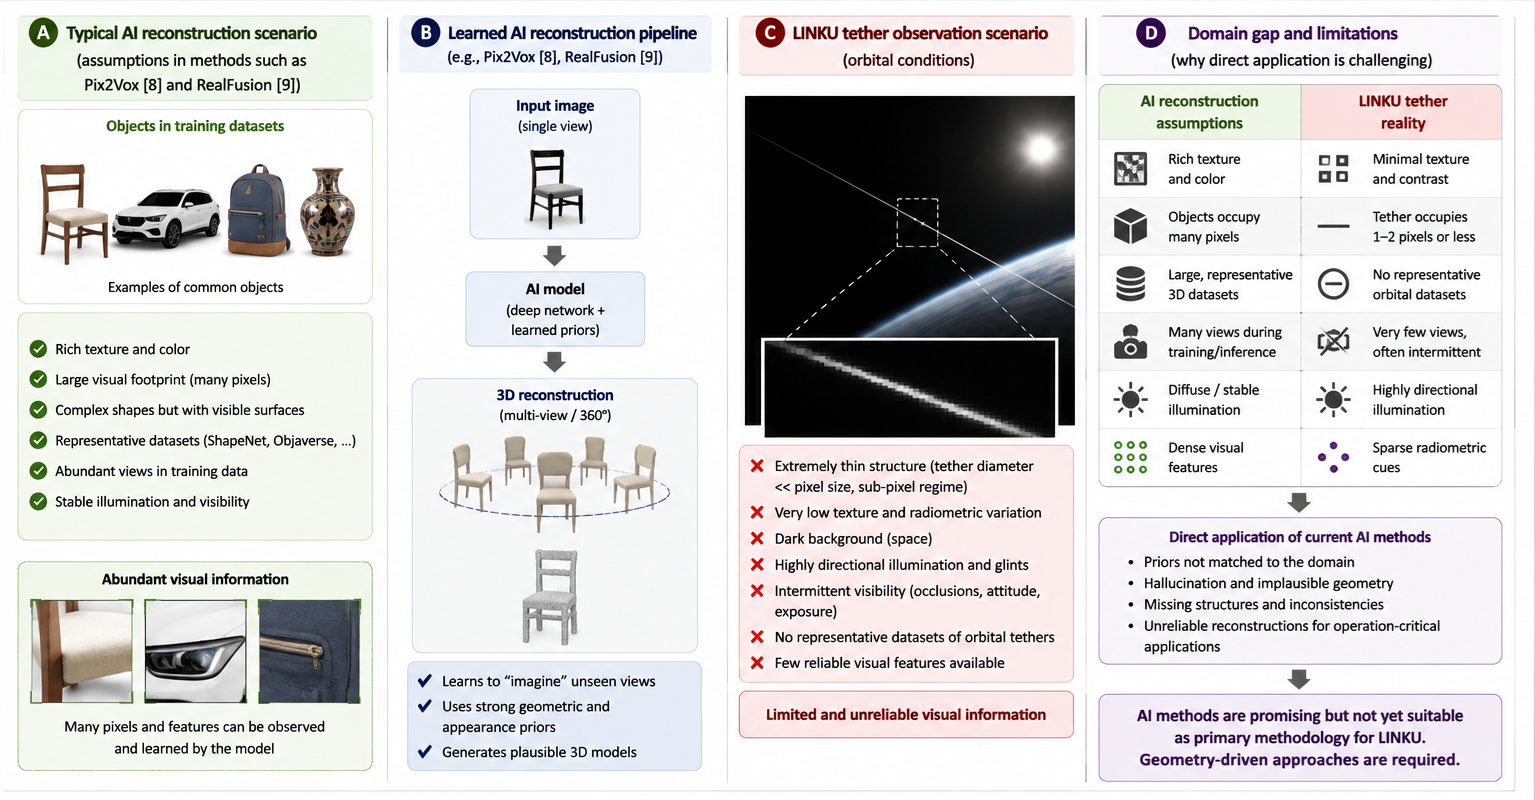
\includegraphics[width=\textwidth]{Images/Figure 2.4.png}
    \caption[Conceptual comparison between the assumptions of modern AI-assisted reconstruction methods and the visual conditions expected for orbital tether observation]{Conceptual comparison between the assumptions of modern AI-assisted reconstruction methods and the visual conditions expected for orbital tether observation. (A) illustrates the rich visual information typically available in AI reconstruction datasets, including textured objects, abundant image features, and representative training samples. (B) summarizes the reconstruction process employed by methods such as Pix2Vox \cite{xie2019pix2vox} and RealFusion \cite{melas2023realfusion}, where learned geometric priors are used to infer complete three-dimensional object representations from one or multiple images. (C) presents the LINKU observation scenario, characterized by an extremely thin tether observed under sub-pixel conditions, directional illumination, low texture, and limited visual information. (D) highlights the resulting domain gap, showing that the assumptions underlying current AI reconstruction methods differ significantly from the orbital tether observation problem. Consequently, LINKU adopts a deterministic geometry-driven reconstruction framework as its primary operational methodology, while AI-assisted approaches are considered future augmentation mechanisms.}
    \label{fig:figure2.4}
\end{figure}
\newpage
\clearpage

\section{Motivation for the LINKU approach}

The analysis presented throughout this chapter reveals a consistent technological gap in the observation of tethered systems in orbit.
\\\\
Previous missions demonstrated the operational feasibility and scientific relevance of tethered satellite architectures, but they lacked dedicated systems capable of directly reconstructing tether geometry during flight operations. At the same time, conventional photogrammetry techniques remain strongly dependent on texture-based correspondence assumptions that are incompatible with the expected optical conditions of orbital tether observation.
\\\\
Although emerging AI-based methods offer promising future capabilities, their dependence on representative datasets and high computational requirements currently limits their direct applicability to this problem.
\\\\
In response to these limitations, the LINKU project proposes a specialized stereo reconstruction strategy focused specifically on the geometric characteristics of thin tether structures under high-contrast orbital-like illumination conditions.
\\\\
Rather than relying primarily on textured feature matching, the proposed approach prioritizes:
\begin{itemize}
    \item Geometric continuity
    \item Radiometric contrast
    \item Centerline estimation
    \item Stereo geometric constraints
\end{itemize}

This methodology forms the foundation of the LINKU reconstruction pipeline and motivates the experimental validation strategy presented in the following chapters.
